\begin{center}
\usetikzlibrary{intersections}
\usetikzlibrary{patterns}
\usetikzlibrary{positioning,shapes.geometric,shapes.symbols,shapes.misc,shapes.multipart}
\usetikzlibrary{trees}

\tikzset{
	%Diagrammes style
	macro/.style={
		draw,
		rectangle split,
		minimum width=1.5cm,
		rectangle split horizontal,
		rectangle split parts=3,
		minimum height=1.5cm,
		align=center,
		every two node part/.style={align=center, text width=5cm},
		fill=red!30,
	},
    start-end/.style={
        draw,
        rectangle,
        rounded corners,
		minimum width = 2.5cm,
		minimum height=1.5cm,
		align=center,
		text width=2cm,
    },
	cloud/.style={
		draw,
		draw,
		ellipse,
		minimum width = 5cm,
		minimum height=1.5cm,
		align=center,
		text width=5cm,
	},
    input-output/.style={ % requires library shapes.geometric
        draw,
        trapezium,
        trapezium left angle=60,
        trapezium right angle=120,
		minimum width = 5cm,
		minimum height=1.5cm,
		align=center,
		text width=5cm,
    },
    operation/.style={
        draw,
        rectangle,
		fill=blue!30,
		minimum width = 5cm,
		minimum height=1.5cm,
		align=center,
		text width=5cm,
    },
    loop/.style={ % requires library shapes.misc
        draw,
        chamfered rectangle,
        chamfered rectangle xsep=1.5cm,
		minimum width = 5cm,
		minimum height=1.5cm,
		align=center,
		text width=5cm,
    },
    decision/.style={ % requires library shapes.geometric
        draw,
        diamond,
		aspect=3,
		minimum width = 5cm,
		align=center,
		text width=5cm,
		fill=green!30,
    },
    print/.style={ % requires library shapes.symbols
        draw,
        tape,
        tape bend top=none,
		minimum width = 5cm,
		minimum height=1.5cm,
		align=center,
		text width=5cm,
    },
    connection/.style={
        draw,
        circle,
        radius=5pt,
		node distance=0pt and 0pt,
		text width=0cm,
		align=center,
    },
	emptyConnection/.style={
		draw=none,
		node distance=0cm,
		align=center,
	}
	vectors/.style={
		red,
		<-,
		thick,
	},
	grid/.style={
		gray,
		step=0.5cm,
		very thin,
	},
	probabilityName/.style={
		text width=4em,
		thick,
		text centered,
	}
}

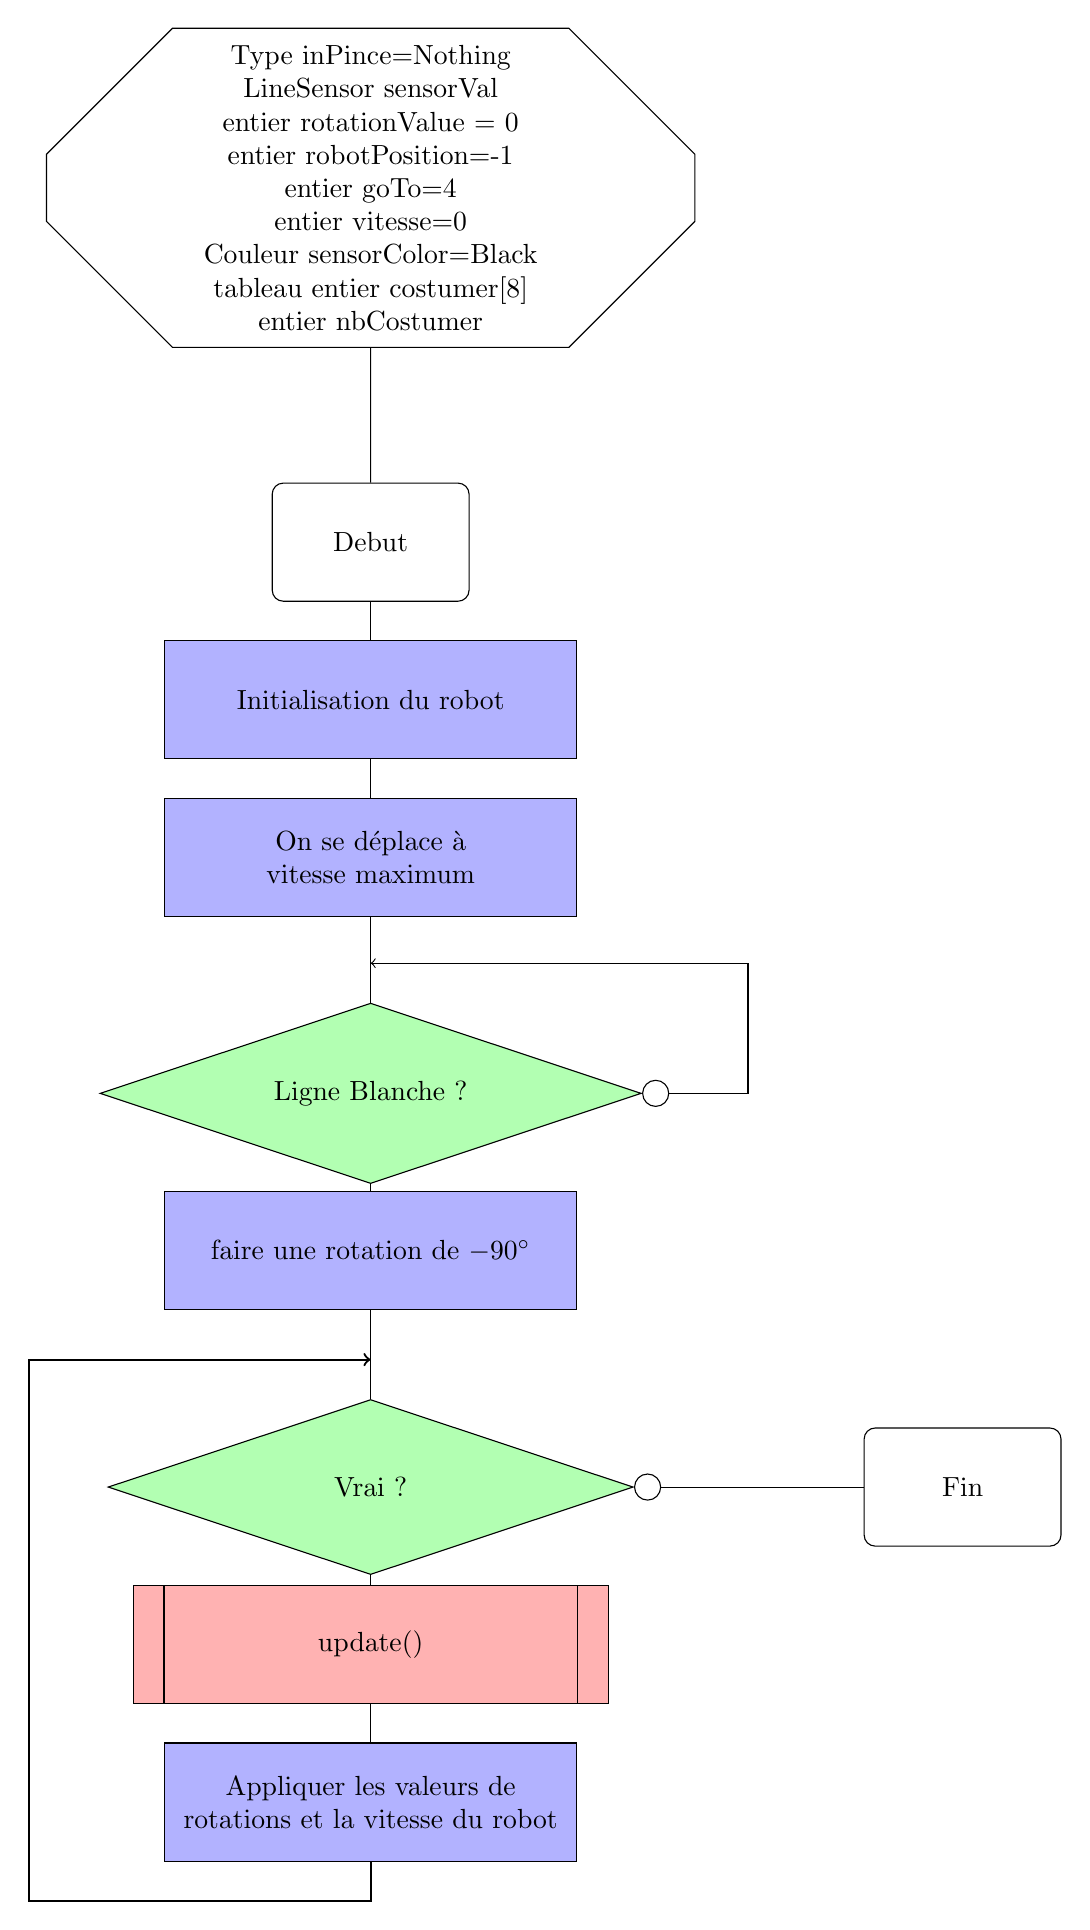
\begin{tikzpicture}[node distance=2cm and 9cm]
	\node(declaration) at (0,0) [loop, align=center] {Type inPince=Nothing \\
	LineSensor sensorVal \\
	entier rotationValue = 0 \\
	entier robotPosition=-1 \\ 
	entier goTo=4 \\
	entier vitesse=0 \\ 
	Couleur sensorColor=Black \\ 
	tableau entier costumer[8] \\ 
	entier nbCostumer};

	\node [below of=declaration, yshift=-2.5cm, start-end] (begin) {Debut} edge (declaration);
	\node [below of=begin, operation] (init) {Initialisation du robot} edge (begin);
	\node [below of=init, operation] (setMotor) {On se déplace à vitesse maximum} edge(init);
	\node [below of=setMotor, yshift=-1cm, decision] (whiteLine) {Ligne Blanche ?} edge (setMotor);
	\node (no) at (whiteLine.east) [connection, text width=0cm, xshift=5pt] {};

	\draw[->] (no.east) -| ([xshift=1cm, yshift=0.5cm]no.east) |- ([yshift=0.5cm]whiteLine.north);

	\node [below of=whiteLine, operation] (rotation) {faire une rotation de $-90^\circ$} edge (whiteLine);
	\node [below of=rotation, yshift=-1cm, decision] (true) {Vrai ?} edge (rotation);
	\node(connection1) at ([xshift=5pt]true.east) [connection] {};
	\node [right of=connection1, start-end, text width=2cm, xshift=2cm] (end) {Fin} edge (connection1);
	\node [below of=true, macro] (update) {
		\nodepart{two}update()} edge(true);
	\node [below of=update, operation] (continue) {Appliquer les valeurs de rotations et la vitesse du robot} edge(update);
	\draw[->, thick] (continue.south) --+ (0,-0.5) -| ([xshift=-1cm]true.west) |- ([yshift=0.5cm]true.north);
\end{tikzpicture}

\newpage

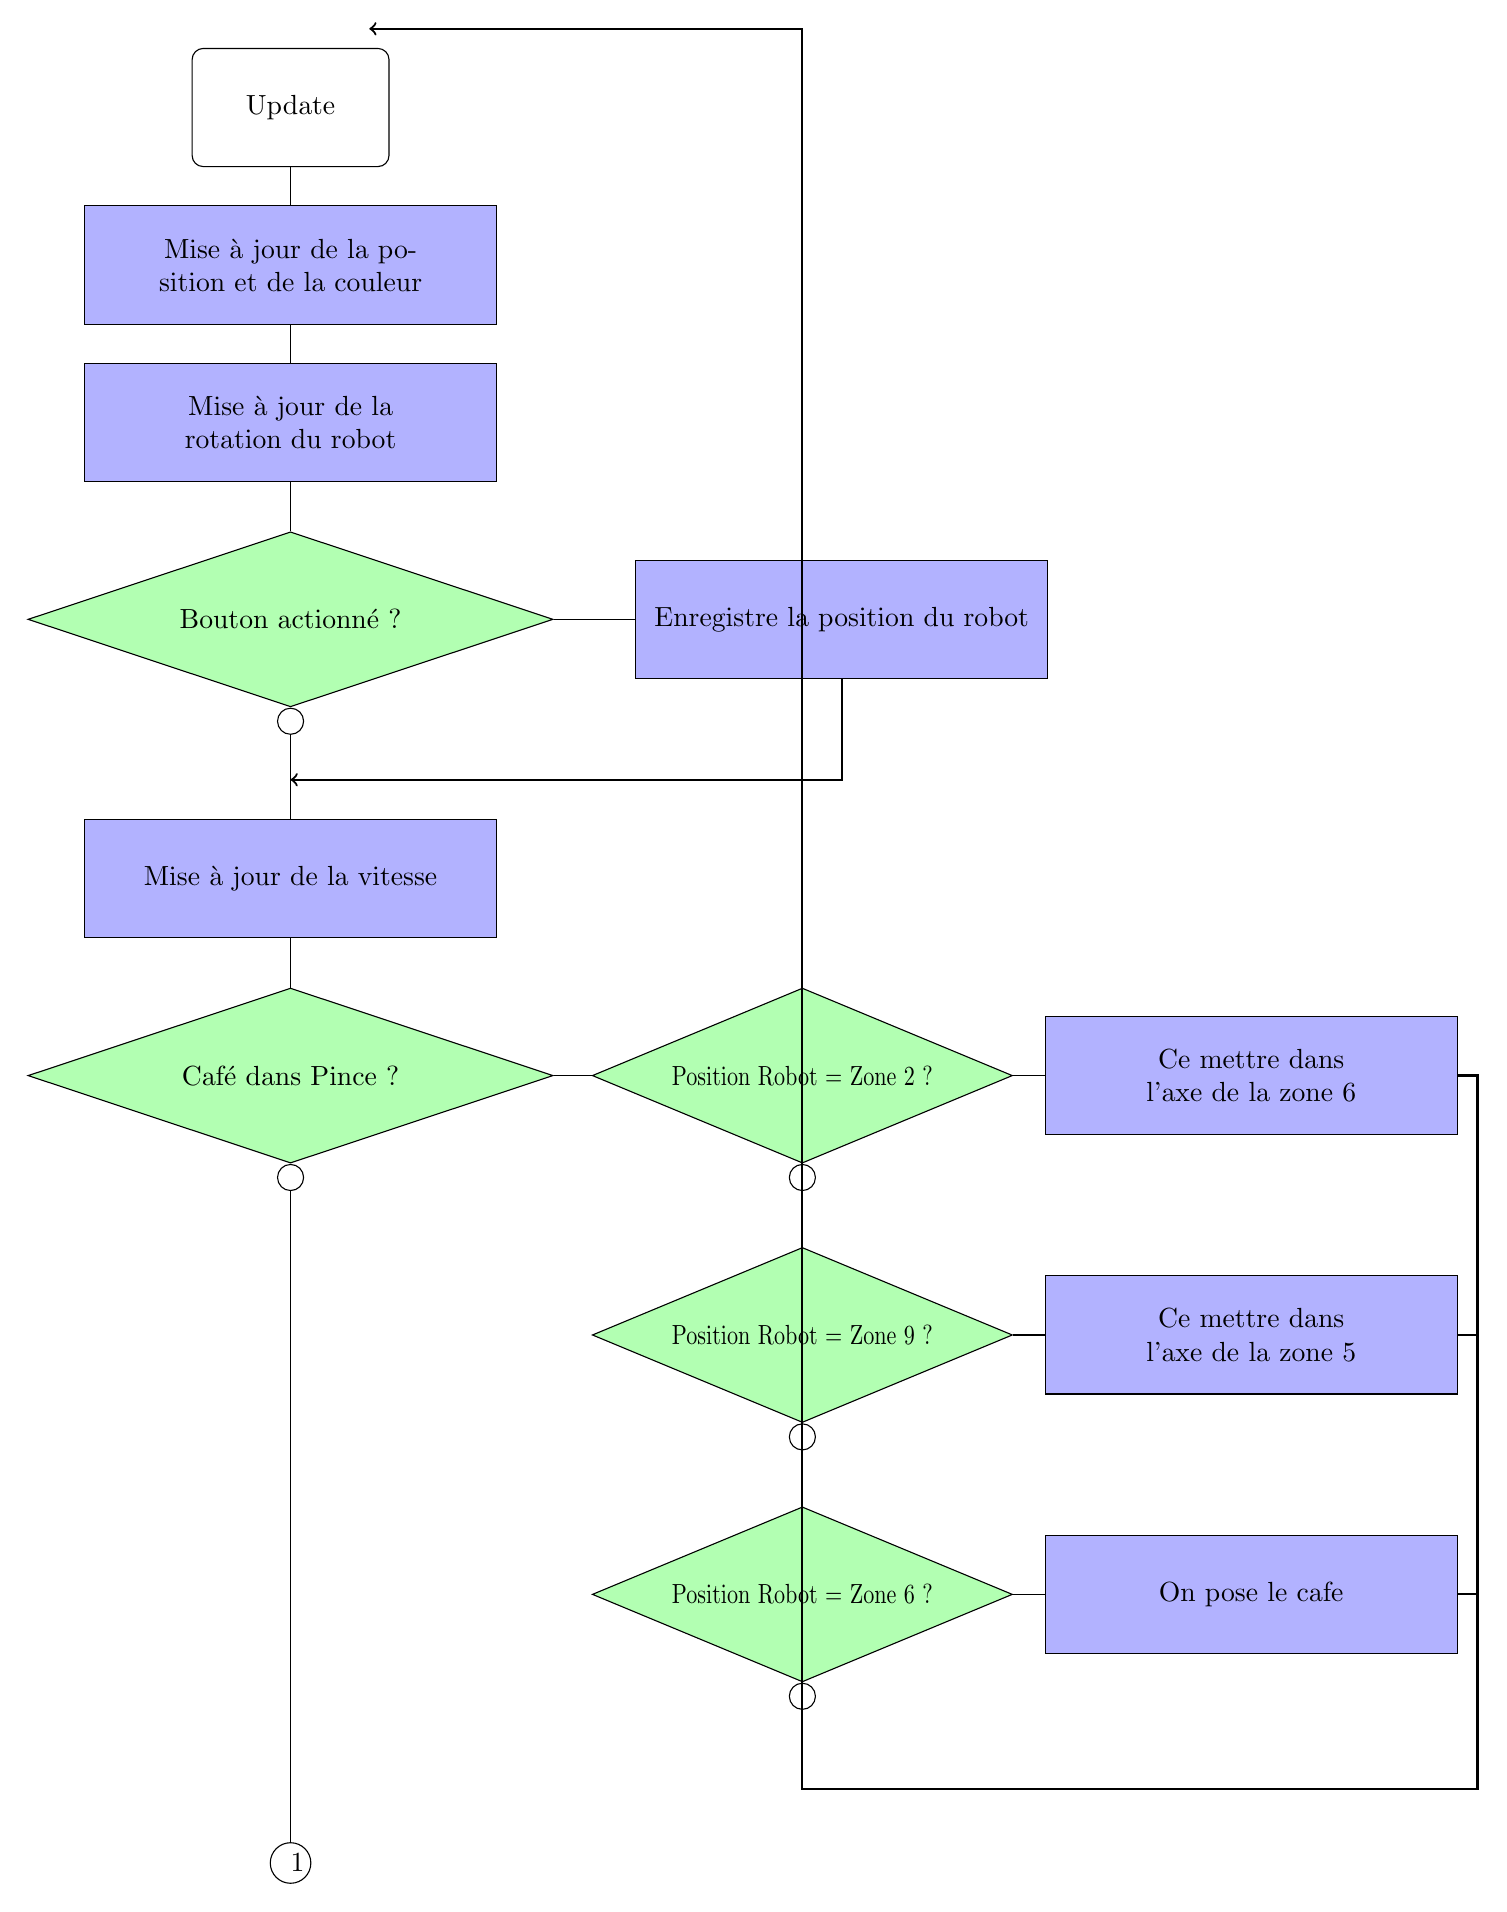
\begin{tikzpicture}[node distance=2cm and 9cm]
	\node(begin) at (0,0) [start-end] {Update};
	\node [below of=begin, operation] (MAJCo) {Mise à jour de la position et de la couleur} edge (begin);
	\node [below of=MAJCo, operation] (MAJR) {Mise à jour de la rotation du robot} edge (MAJCo);
	\node [below of=MAJR, decision, yshift=-0.5cm] (bouton) {Bouton actionné ?} edge (MAJR);
	\node(connection1) at ([yshift=-5pt]bouton.south) [connection] {};
	\node [right of=bouton, operation, xshift=5cm] (enre) {Enregistre la position du robot} edge (bouton);
	\node [below of=connection1, operation] (majv) {Mise à jour de la vitesse} edge (connection1);
	\draw [->, thick] (enre.south) |- ([yshift=0.5cm]majv.north);
	\node [below of=majv, decision, yshift=-0.5cm] (selon) {Café dans Pince ?} edge (majv);
	\node(connection2) at ([yshift=-5pt]selon.south) [connection] {};
	\node [right of=selon, decision, xshift=4.5cm, xscale=0.8] (plusRapide) {Position Robot = Zone 2 ?} edge (selon);
	\node(connection3) at ([yshift=-5pt]plusRapide.south) [connection] {};
	\node[right of=plusRapide, operation, xshift=3.7cm] (tourner) {Ce mettre dans l'axe de la zone 6} edge (plusRapide);

	\node [below of=connection3, decision, xscale=0.8] (versZone) {Position Robot = Zone 9 ?} edge (connection3);
	\node[right of=versZone, operation, xshift=3.7cm] (tourner5) {Ce mettre dans l'axe de la zone 5} edge (versZone);
	\node(connection4) at ([yshift=-5pt]versZone.south) [connection] {};

	\node [below of=connection4, decision, xscale=0.8] (poseCafe) {Position Robot = Zone 6 ?} edge (connection4);
	\node(connection5) at ([yshift=-5pt]poseCafe.south) [connection] {};
	\node [right of=poseCafe, operation, xshift=3.7cm] (pose) {On pose le cafe} edge (poseCafe);

	\getxy{\x}{\y}{connection2.south}
	\coordinate (A) at ([yshift=-1cm]connection5.south);
	\getxy{\xa}{\ya}{A}
	\draw [->, thick] (tourner.east) -- ([xshift=0.25cm]tourner.east) |- ([yshift=-1cm]connection5.south) |- (\x,\ya);
	\node [below of=selon, connection, yshift=-10cm] {1} edge (connection2);
	\draw [thick] (connection5.south) -- ([yshift=-1cm]connection5.south);
	\draw [thick] (tourner5.east) -- ([xshift=0.25cm]tourner5.east);
	\draw [thick] (pose.east) -- ([xshift=0.25cm]pose.east);
\end{tikzpicture}

\newpage

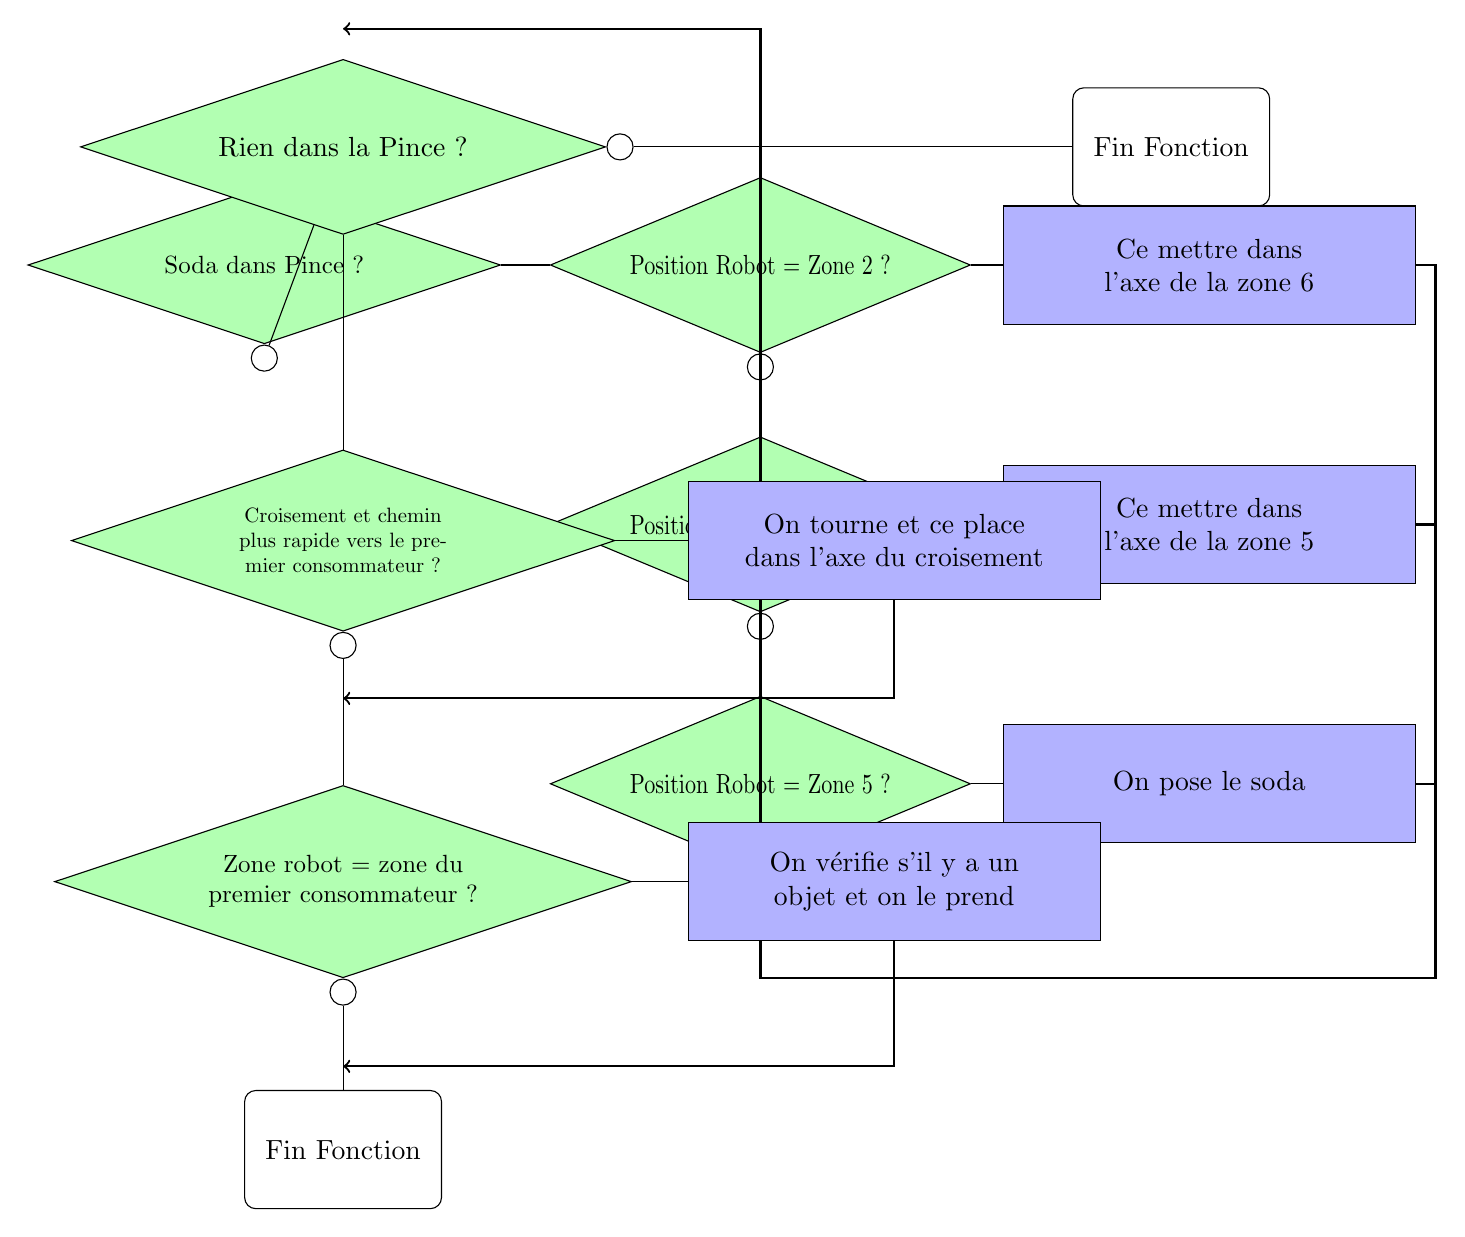
\begin{tikzpicture}[node distance = 2cm and 9cm]
	\node(begin) at (0,0) [connection] {1};
	\node[below of=begin, decision, scale=0.9] (pinceSoda) {Soda dans Pince ?} edge (begin);
	\node(connection) at ([yshift=-5pt]pinceSoda.south) [connection] {};

	\node [right of=pinceSoda, decision, xshift=4.3cm, xscale=0.8] (zone2) {Position Robot = Zone 2 ?} edge (pinceSoda);
	\node(connection2) at ([yshift=-5pt]zone2.south) [connection] {};
	\node[right of=zone2, operation, xshift=3.7cm] (tourner) {Ce mettre dans l'axe de la zone 6} edge (zone2);

	\node [below of=connection2, decision, xscale=0.8] (versZone) {Position Robot = Zone 9 ?} edge (connection2);
	\node[right of=versZone, operation, xshift=3.7cm] (tourner5) {Ce mettre dans l'axe de la zone 5} edge (versZone);
	\node(connection3) at ([yshift=-5pt]versZone.south) [connection] {};

	\node [below of=connection3, decision, xscale=0.8] (poseSoda) {Position Robot = Zone 5 ?} edge (connection3);
	\node(connection4) at ([yshift=-5pt]poseSoda.south) [connection] {};
	\node [right of=poseSoda, operation, xshift=3.7cm] (pose) {On pose le soda} edge (poseSoda);

	\getxy{\x}{\y}{connection.south}
	\coordinate (A) at ([yshift=-1cm]connection4.south);
	\getxy{\xa}{\ya}{A}
	\draw [->, thick] (tourner.east) -- ([xshift=0.25cm]tourner.east) |- ([yshift=-1cm]connection4.south) |- (\x,\ya);
	\draw [thick] (connection4.south) -- ([yshift=-1cm]connection4.south);
	\draw [thick] (tourner5.east) -- ([xshift=0.25cm]tourner5.east);
	\draw [thick] (pose.east) -- ([xshift=0.25cm]pose.east);

	\coordinate (B) at (\x,\ya);
	\node (pinceN) at ([yshift=-1.5cm]B) [decision] {Rien dans la Pince ?} edge (connection);
	\node (connectionEnd) at ([xshift=5pt]pinceN.east) [connection] {};
	\node [right of=connectionEnd, xshift=5cm, start-end] (end) {Fin Fonction} edge (connectionEnd);

	\node [below of=pinceN, yshift=-3cm, decision, scale=0.75] (decisionRapide) {Croisement et chemin plus rapide vers le premier consommateur ?} edge (pinceN);
	\node [right of=decisionRapide, xshift=5cm, operation] (cheminRapide) {On tourne et ce place dans l'axe du croisement} edge (decisionRapide);
	\node(connection5) at ([yshift=-5pt]decisionRapide.south) [connection] {};

	\draw[->, thick] (cheminRapide.south) |- ([yshift=-0.5cm]connection5.south);
	\node[below of=connection5, yshift=-1cm, decision, scale=0.9] (consommateur) {Zone robot = zone du premier consommateur ? } edge (connection5);
	\node[right of=consommateur, operation, xshift=5cm] (debarasser) {On vérifie s'il y a un objet et on le prend} edge (consommateur);
	\node(connection6) at ([yshift=-5pt]consommateur.south) [connection] {};

	\node [below of=connection6, start-end] (end2) {Fin Fonction} edge (connection6);
	\draw[->, thick] (debarasser.south) |- ([yshift=0.3cm]end2.north);
\end{tikzpicture}

\end{center}
